\ifx\papersnotes\undefined
    \providecommand{\notesroot}{../..}
    \providecommand{\nlppapersroot}{.}

    \title{自然语言处理}
    \author{Donald Cheung\\jianzhang9102@gmail.com}
    \date{\today\footnote{文档编写开始于2018年5月17日}}

    \documentclass[a4paper,10pt]{ctexbook}
\usepackage{xeCJK}
\usepackage{fontspec}
\usepackage{minted}
\usepackage[CJKbookmarks,colorlinks,linkcolor=red]{hyperref}
\usepackage{geometry}
\usepackage{amsmath}
\usepackage[format=hang,font=small,textfont=it]{caption}
\usepackage{float}
\usepackage{subfigure}
\usepackage[nottoc]{tocbibind}
\usepackage{bm}
\usepackage[table, x11names, dvipsnames]{xcolor}
\usepackage{color}
\usepackage{array, booktabs, boldline}
\usepackage{cellspace}
\usepackage{longtable}

\setmainfont{Times New Roman}
\setsansfont{Helvetica}
\setmonofont{Courier New}
\setCJKmainfont[BoldFont={SimHei},ItalicFont={SimHei}]{SimSun}
\setCJKsansfont{SimSun}
\setCJKmonofont{SimSun}

\setcounter{secnumdepth}{4}
\setcounter{tocdepth}{4}

\geometry{left=3.0cm,right=3.0cm,top=2.5cm,bottom=2.5cm}
\bibliographystyle{plain}

%%%%%%%%%%%%%%%%%%%%%%%%%%%%%%%%% minted setting %%%%%%%%%%%%%%%%%%%%%%%%%%%%%%%%%%%
\usemintedstyle{monokai}
\definecolor{bg}{HTML}{282828} % from https://github.com/kevinsawicki/monokai
%\defaultfontfeatures{}
\newfontfamily\noligsmonofamily[NFSSFamily=noligsmonofamily]{Courier}
\setminted{fontfamily=noligsmonofamily}

\renewcommand{\theFancyVerbLine}{%
    \sffamily \textcolor{Dandelion}{\scriptsize \oldstylenums{\arabic{FancyVerbLine}}}}

\newenvironment{jcode}[3]
{%
    \VerbatimEnvironment
    \begin{listing}[h]%
    \caption{#2}%
    \label{#3}%
    \begin{minted}[xleftmargin=18pt,
                   mathescape,
                   linenos,
                   numbersep=5pt,
                   bgcolor=bg,
                   frame=lines,
                   framesep=2mm,
                   fontsize=\footnotesize]{#1}%
}
{%
    \end{minted}
    \vspace{-25pt}%
    \end{listing}%
}
\renewcommand{\listingscaption}{代码}%from minted
\renewcommand{\listoflistingscaption}{代码列表}% from minted


\newenvironment{myquote}{\begin{quote}\kaishu\zihao{-5}}{\end{quote}}
\newcommand\degree{^\circ}
\newtheorem{thm}{定理}


\begin{document}
\maketitle
\tableofcontents
\listoflistings

\else
    \providecommand{\nlppapersroot}{\papersroot/nlp}
\fi

\chapter{自然语言处理}

\section{句子对匹配}

\subsection{A Decomposable Attention Model for Natural Language Inference \cite{parikh2016decomposable}}

\subsubsection{问题介绍}
Natural language inference,自然语言推断。其实就是文本蕴含任务(text entailment),任务的形式是:
给定一个前提文本(premise),根据这个 premise 去推断假说文本(hypothesis)与 premise 的关系,
一般分为蕴含关系(entailment)和矛盾关系(contradiction),
蕴含关系(entailment)表示从 premise 中可以推断出 hypothesis;
矛盾关系(contradiction)即 hypothesis 与 premise 矛盾。


这篇论文的实验是用的SNLI数据集。

\subsubsection{主要方法}
每个训练数据由三个部分组成 $\left\{ a^{(n)}, b^{(n)}, y^{(n)} \right\}_{n=1}^{N}$,
模型的输入为 $a = (a_{1}, \cdots, a_{l_{a}})$ 和 $b = (b_{1}, \cdots, b_{l_{b}})$,分别代表前提和假说,
$y^{(n)}=\left( y_{1}^{(n)}, \cdots, y_{C}^{(n)} \right)$ 表示 $a$ 和 $b$ 之间的关系标签,
$C$ 为输出类别的个数,因此 $y $是个 $C$ 维的 $0,1$ 向量。
训练目标就是根据输入的 $a$ 和 $b$ 正确预测出他们的关系标签 $y$。

整个模型如图所示,整体分为三个部分:Attend, Compare, Aggregate。

\begin{figure}[H]
  \centering
  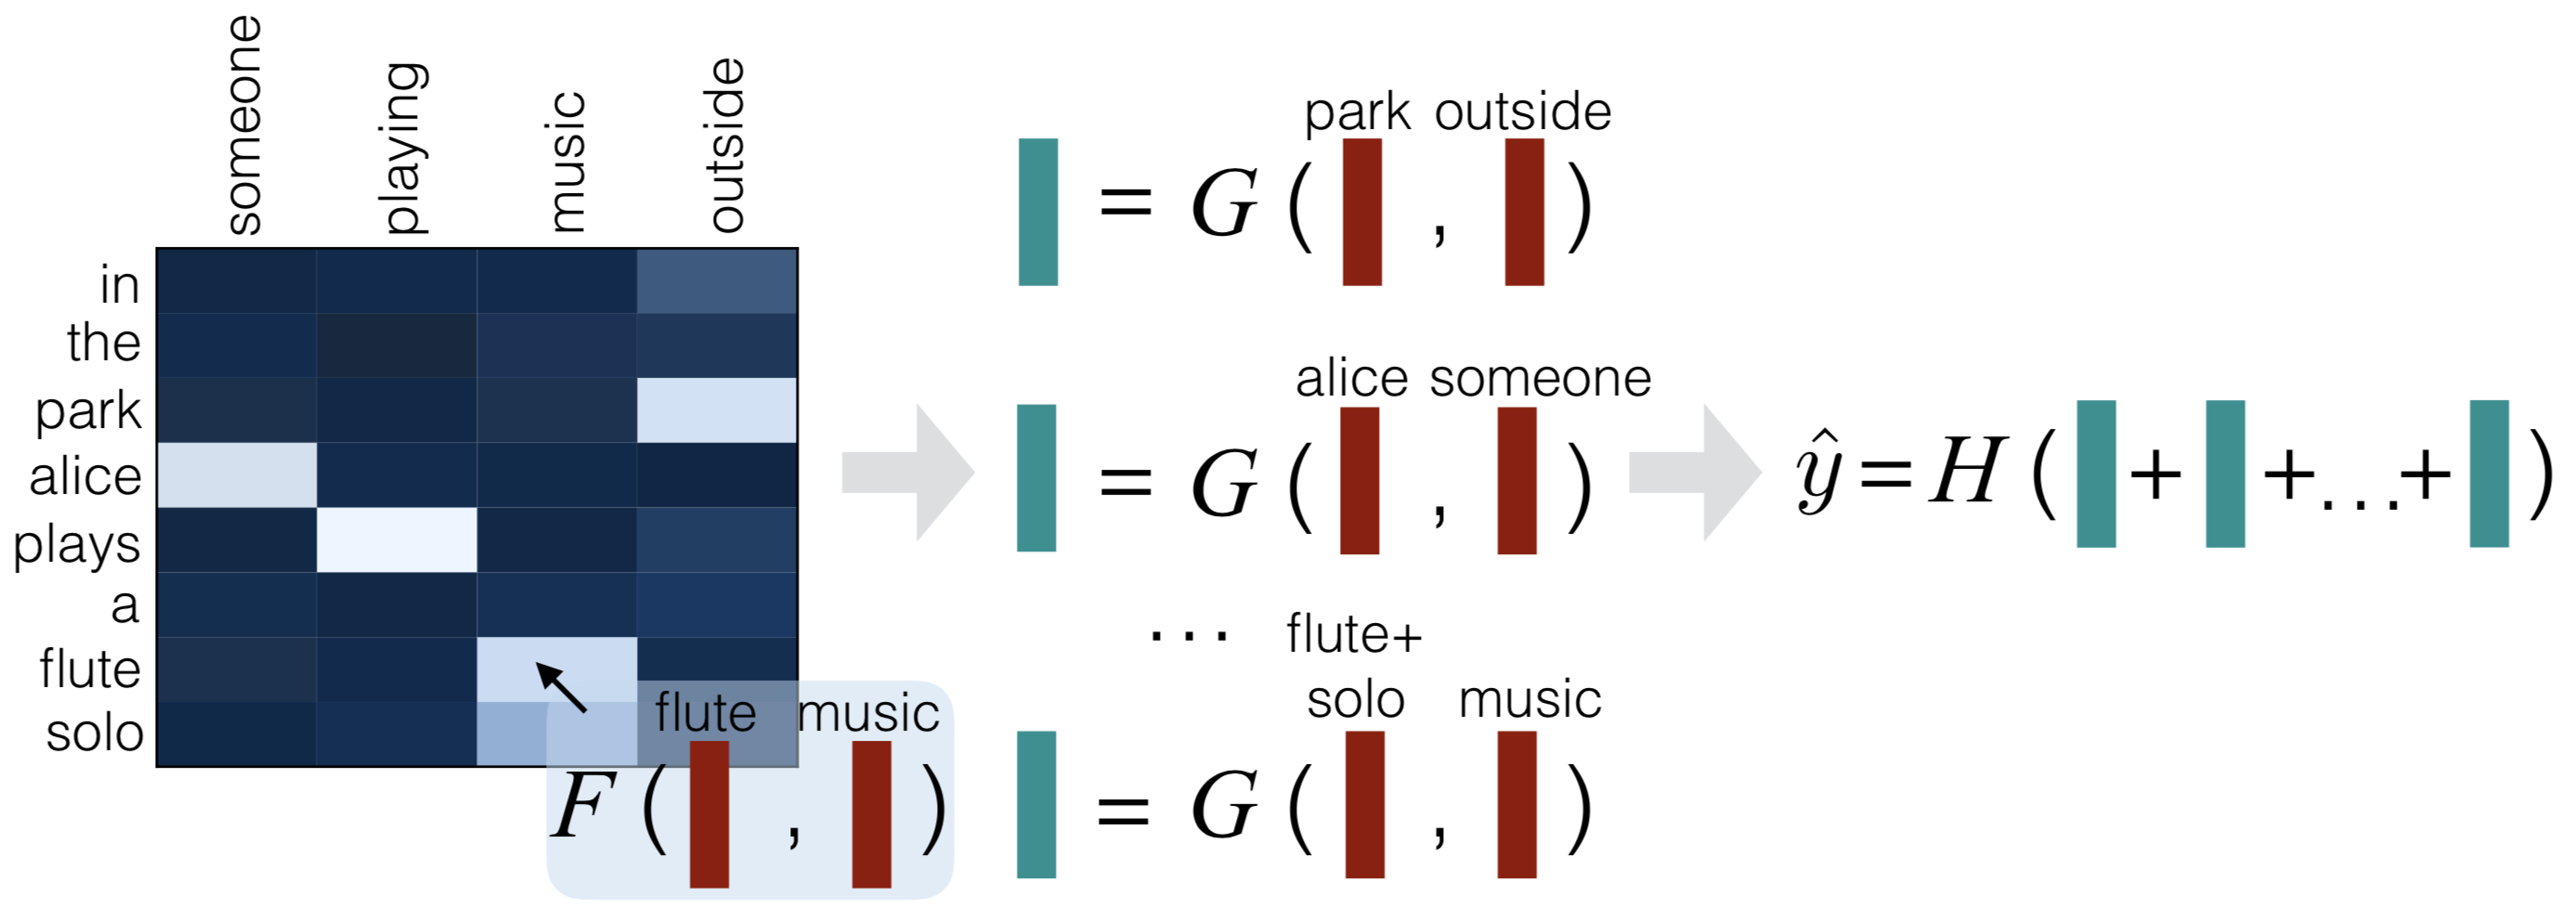
\includegraphics[scale=0.25]{\nlppapersroot/images/Parikh-2016aa-Model.png}
  \caption{Decomposable 模型整体结构}
  \label{fig:Parikh-2016aa-Model}
\end{figure}

假设 $\overline{a} = (\overline{a}_1, \cdots, \overline{a}_{l_a})$ 和
$\overline{b} = (\overline{b}_1, \cdots, \overline{b}_{l_b})$ 分别表示两个输入句子的表示。
例如,最简单的表示方式就是 $\overline{a} = a$ 和 $\overline{b} = b$。
这种方式没有用到词序的信息,可以将词的位置信息也做 Embedding 作为模型的输入。

\begin{enumerate}
    \setcounter{enumi}{-1}
    \item Projection

        对输入的词向量进行投射,投射到另一个维度。例如,词向量的维度是300维,此步操作将其投射到200维,
        投射的权重也为参数,需要进行训练。当然,也可以没有这部分操作,直接使用输入的词向量。

    \item Attend

        此步是计算 $a$ 和 $b$ 之间每两个词之间的 attention weights $e_{ij}$。
        $e_{ij}$ 可以用函数 $F'$ 来计算,即 $F'(\overline{a}, \overline{b})$。
        如果此时 $F'$ 用前向的神经网络来表示的话,则一次 attention weights 的计算
        需要前向计算神经网络 $\ell_a \times \ell_b$ 次,开销比较大。可以将这部分的计算拆解为以下的形式:
        \[
            e_{ij} = F'(\overline{a}_i, \overline{b}_j) = F(\overline{a}_i)^{T} F(\overline{b}_j)
        \]
        同样,$F$ 可以用前向的神经网络计算,但此时只需要计算 $\ell_a + \ell_b$ 次前向的神经网络即可。

        拿到 attention weights 之后,计算每个词与对方句子中所有词的软对齐即可,具体对齐向量的计算如下:
        \begin{align*}
            \beta_i = \sum_{j=1}^{\ell_b} \frac{exp(e_{ij})}{\sum_{k=1}^{\ell_b}{exp(e_{ik})}} \overline{b}_j , \\
            \alpha_j = \sum_{i=1}^{\ell_a} \frac{exp(e_{ij})}{\sum_{k=1}^{\ell_a}{exp(e_{kj})}} \overline{a}_i.
        \end{align*}
        其中,$\beta_i$ 是 $\overline{b}$ 中与 $\overline{a}_i$ 软对齐的向量,$\alpha_j$ 则相反。

    \item Compare

        此步的功能主要是将一个句子与其在另一个句子中的软对齐向量做比较,即:
        \begin{align*}
            \mathbf{v}_{1,i} = G([\overline{a}_i, \beta_i]) \qquad \forall i \in [1, \cdots, \ell_a], \\
            \mathbf{v}_{2,j} = G([\overline{b}_j, \alpha_j]) \qquad \forall j \in [1, \cdots, \ell_b]
        \end{align*}

        其中, $[\cdot, \cdot]$ 表示两个向量做拼接。$G$ 同样可以使用前向的神经网络来计算。

    \item Aggregate

        在拿到了两个句子的对比向量 $\left\{\mathbf{v}_{1,i}\right\}_{i=1}^{\ell_a}$ 和
        $\left\{\mathbf{v}_{2,j}\right\}_{j=1}^{\ell_b}$ 之后,此步对每个句子的对比向量汇总求和:
        \[
            \mathbf{v}_{1}=\sum_{i=1}^{\ell_a} \mathbf{v}_{1,i} \qquad,\qquad 
            \mathbf{v}_{2}=\sum_{j=1}^{\ell_b} \mathbf{v}_{2,j}
        \]

        拿到汇总后的两个向量之后,将结果输入到神经网络 $H$ 即可,
        $H$ 为一个前向的神经网络并在最后接一个线性的网络层。
        \[
            \hat{\mathbf{y}} = H([\mathbf{v}_1, \mathbf{v}_2]),
        \]
        其中,$\hat{\mathbf{y}} \in \mathbb{R}^{C}$ 为每个类别的预测分数(未归一化),
        从而最终预测的类为 $\hat{y} = \arg\max_{i}{\hat{\mathbf{y}}_i}$.

    \item Intra-Sentence Attention(优化)

\end{enumerate}


训练时采用交叉熵作为误差损失函数,并使用dropout:
\[
    L(\theta_F, \theta_G, \theta_H) = \frac{1}{N}\sum_{n=1}^{N}\sum_{c=1}^{C}
                                    {y_c^{(n)} \log \frac{exp(\hat{y}_c)}{\sum_{c'=1}^{C}{exp(\hat{y}_{c'})}}}
\]
其中 $\theta_F, \theta_G, \theta_H$ 代表模型的参数。


\subsubsection{实验验证}
待补充


\subsubsection{相关材料和笔记}
\begin{enumerate}
    \item \href{https://zhuanlan.zhihu.com/p/26237357}{《A Decomposable Attention Model for Natural Language Inference》阅读笔记}
    \item \href{https://pdfs.semanticscholar.org/2c3a/1947e2635d6be3da8a3cf06f137847a1cc02.pdf}{slides}
    \item \href{https://towardsdatascience.com/convolutional-attention-model-for-natural-language-inference-a754834c0d83}{
                    Convolutional Attention Model for Natural Language Inference}
\end{enumerate}


\subsubsection{相关实现}
\begin{enumerate}
    \item Harvard基于torch实现的版本:\url{https://github.com/harvardnlp/decomp-attn}

    \item Decomposable和优化版论文 \cite{chen2017enhanced} 的实现:\url{https://github.com/erickrf/multiffn-nli}

\end{enumerate}

\ifx\papersnotes\undefined
    \bibliography{\notesroot/reference/reference.bib}
\end{document}

\fi
